\documentclass[../main.tex]{subfiles}
\begin{document}
\section{模型建立和求解}
\subsection{问题1的模型建立和求解}
\subsubsection{模型准备}
%%
\paragraph{太阳高度角和太阳方位角}
记 \(\alpha _{s}\) 为太阳高度角,\(\gamma _{s}\)为太阳方位角。已知:
\begin{equation}
\sin \alpha _{s} = \cos \delta \cos \varphi \cos \omega + \sin \delta \sin \varphi\label{equ:alpha},
\end{equation}
\begin{equation}
\cos \gamma _{s} = \frac{\sin \delta -\sin \alpha_{s} \sin \varphi}{\cos \alpha _{s} \cos \varphi}\label{equ:gamma}
\end{equation}
记 \( \varphi\) 为纬度,\(\omega\) 为太阳时角,\(ST\) 为当地时间, \(\delta\) 为太阳赤纬角,有
\begin{equation}
\omega = \frac{\pi}{12} ( ST - 12),
\end{equation}
\begin{equation}
\sin \delta = \sin \frac{2 \pi D}{365} \sin \big(\frac{2\pi}{360} \cdot 23.45\big),
\end{equation}
设太阳中心发出的光线的方向向量为 \(\vec\lambda _{i} = (x,  y , z)\)。若将\(\vec \lambda_{i}\)单位化,有
\begin{equation}
\vec \lambda _{i} = ({-} \cos \alpha _{s} \sin \gamma_{s} ,{-} \cos \alpha_{s} \cos \gamma_{s}, {-} \sin \alpha_{s})
\end{equation}
%%
\paragraph{太阳半角展宽的推导}
由题意,太阳光不应考虑为平行光,而应当建模为具有锥形角的锥形光束,以下对锥形的半角展宽 \( \alpha_{h}\)的推导。如图
%
\begin{figure}[H]
\centering
\input fig_earth_sun.tex
\caption{\kaishu 太阳半角展宽求解示意图}
\end{figure}
%
由几何关系可知
\begin{equation}
\sin \alpha_{h} = \frac{R_{2}}{R_1 - R_3}
\end{equation}
经查阅资料\cite{abook}可知
,\(R_1 = 1.496\times 10 ^{8} \, \mathrm{km}\),\(R_2 = 6.963\times 10 ^{5}\,\mathrm{km}\),\(R_3 = 3.959\times 10^{3}\, \mathrm{km}\),代入上式计算得
\begin{equation}
\alpha_{h} \approx 4.65 \mathrm{mrad} \approx 0.5 ^{\circ}
\end{equation}
%%
\paragraph{相关公式}
法向直接辐射照度 DNI 按照下面公式近似计算:
\begin{equation}
\begin{aligned}
\mathrm{DNI} = G_{0} \bigg[ a + b \cdot \exp\Big\{{-}\frac{c}{\sin \alpha_{s}}\Big\}\bigg]\\
a = 0.4237 + 0.00821 (6 - H) ^{2} \\
b = 0.5055 + 0.00595(6.5 - H) ^{2} \\
c = 0.2711 + 0.01858 (2.5 - H) ^{2}
\end{aligned}
\end{equation}
其中 \(G_{0}\) 是太阳常数。镜场的输出热功率为 \(E_{\mathrm{field}}\) 为
\begin{equation}
E_{\mathrm{field}} = \mathrm{DNI} \cdot \sum _{i} ^{N} A_{i} \eta _{i}
\end{equation}
定日镜光学效率\(\eta\)为
\begin{equation}
\eta = \eta _{\mathrm{s b}} \eta _{\cos} \eta _{\mathrm{at}} \eta _{\mathrm{trunc}} \eta _{\mathrm{ref}},
\end{equation}
其中 \(\eta _{\mathrm{s b}}\) 为阴影遮挡效率。阴影遮挡损失是指由于阴影或者是遮挡导致的效率损失,\(\eta _{\cos}\) 是余弦效率,大气透射率 \(\eta _{\mathrm{at}}\) 由下面公式确定:
\begin{equation}
\eta _{\mathrm{at}} = 0.99321 - 0.0001176 d _{\mathrm{HR}} + 1.97 \times 10 ^{-8} \times d _{\mathrm{HR}} ^{2},
\end{equation}
其中 \(d _{\mathrm{HR}}\)是镜面中心到集热器中心的距离。截断效率为\(\eta _{\mathrm{trunc}}\) 。因为部分反射光束没有照射到中心塔塔顶的集热器导致效率损失。

设入射光线为 \(\vec S\),反射光线为 \(\vec R\),余弦效率使用下面公式计算:
\begin{equation}
\eta _{\cos} = \cos \big(\arccos (\vec R \cdot \vec S) / 2\big)
\end{equation}
%%
\paragraph{旋转矩阵}
已知地面坐标系 \(x y z\)以圆形区域的圆心为原点,正北方向为 \(y\) 轴正方向,正东方向为 \(x\) 轴正方向,垂直地面向上的方向为 \(z\) 轴正方向。假设已知一个定日镜的镜面中心在地面坐标系的坐标 \(N = (x_0,  y_0 , d)\),其中 \(d\) 是安装高度,现在以定日镜镜面中心为坐标原点,镜面法向为 \(z\) 轴,如图所示建立坐标系,记为 \(x'y'z'\)。

设 \(\vec n\) 为该镜面的法向量,方向向外,\(\theta\) 为 \(\vec n\) 和 竖直方向上的夹角,\(\varphi\) 是 \(\vec n\) 水平方向和正东方向的夹角。可以得到坐标变换的公式:
\begin{equation}
\begin{pmatrix}
x_{1}\\
y_1\\
z_1
\end{pmatrix}
= M
\begin{pmatrix}
x_2\\
y_2\\
z_2
\end{pmatrix} +
\begin{pmatrix}
x_0\\
y_0\\
d
\end{pmatrix},
\end{equation}
其中 \((x_2,y_2,z_2)\) 是镜面坐标系里点的坐标,\((x_1,y_1,z_1)\) 是地面坐标系里点的坐标,\(M\) 是旋转矩阵,其为
\[
M  = M_1 M_2,
\]
\begin{figure}
\centering
\input trans.tex
\caption{\kaishu 坐标系变换示意图}
\end{figure}
其中沿纵向转轴旋转角$\theta$对应的旋转矩阵为
\[M_1 = 
\begin{pmatrix}
\cos\theta & -\sin \theta & 0\\
\sin\theta& \cos\theta & 0\\
0&0&1
\end{pmatrix},
\]
沿水平转轴旋转角$\varphi$对应的旋转矩阵为
\[M_2 = 
\begin{pmatrix}
1 & 0 & 0\\
0&\cos\varphi & -\sin\varphi\\
0&\sin\varphi&\cos\varphi
\end{pmatrix},
\]
于是
\begin{equation}\label{equ:transM}
M =
% \begin{pmatrix}
% \cos \theta & - \sin \theta & 0 \\
% \sin \theta & \cos \theta & 0\\
% 0 & 0 & 1
% \end{pmatrix} \cdot
% \begin{pmatrix}
% 1 & 0 & 0\\
% 0 & \cos \varphi & - \sin \varphi\\
% 0 & \sin \varphi & \cos \varphi
% \end{pmatrix}
% =
\begin{pmatrix}
\cos \theta & - \cos \varphi & \sin \varphi \sin \theta\\
\sin \theta & \cos \varphi \cos \theta & - \sin \varphi \cos \theta\\
0 & \sin \varphi & \cos \varphi
\end{pmatrix}
\end{equation}
特别地,当 \(\theta = 0\) 的时候,旋转矩阵 \(M\) 退化为单位矩阵。
于是使用定日镜 \(A\)上一点在镜面坐标系 \(x'y'z'\) 的坐标 \(N_{A}\) \((x_{A}, y_{A},0)\),可知其在地面坐标系之中的坐标\(N\) \((x, y , z)\):
\begin{equation}
\begin{pmatrix}
x\\
y\\
z
\end{pmatrix}
=
\begin{pmatrix}
x_{A} \cos \varphi - y_{A} \cos \varphi \sin \theta + x_0\\
x_{A} \sin \theta + y_{A} \cos \varphi \cos \theta + y_{0} \\
y_{A} \sin \varphi + d
\end{pmatrix}
\end{equation}


\subsubsection{模型建立}
\paragraph{镜场的布局确定} 通过问题所给的附件中关于定日镜的位置信息,绘出定日镜在定日镜场中的排布如下:
%
\begin{figure}[H]
\centering
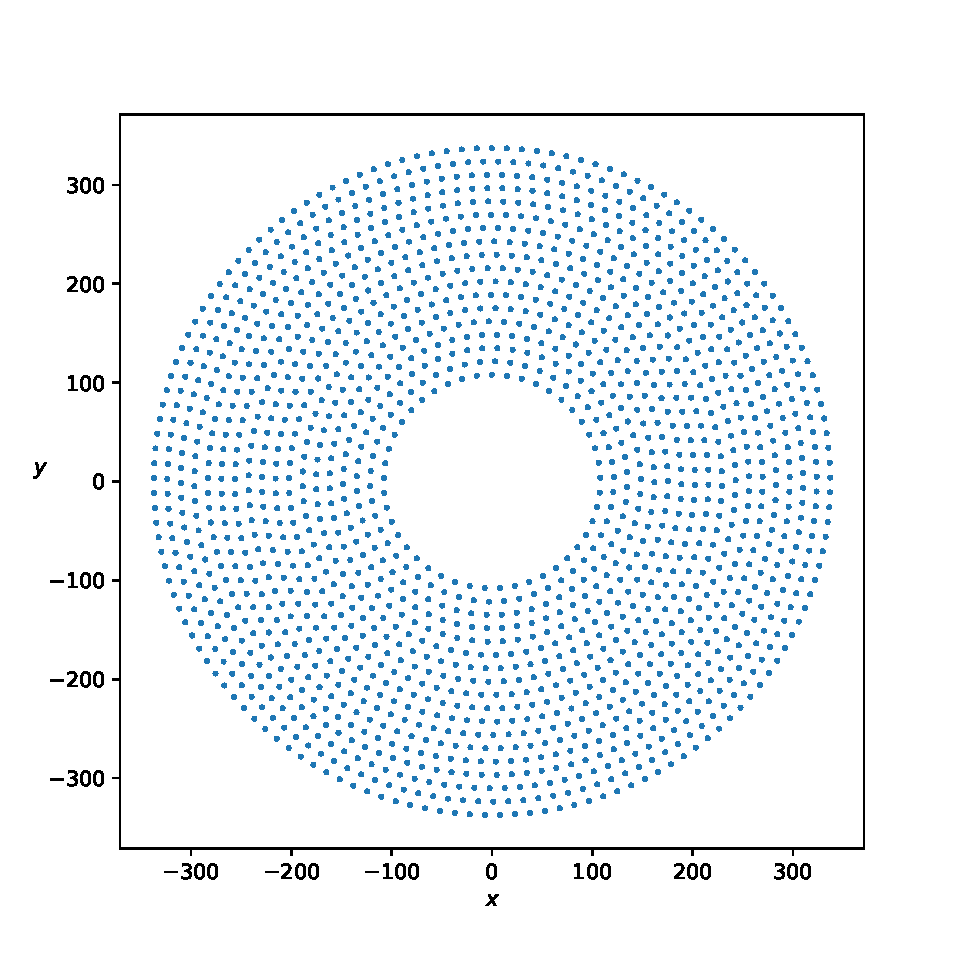
\includegraphics[scale = 0.5]{arange_1.pdf}
\caption{\kaishu 定日镜布局}\label{arange_1}
\end{figure}
%
从该图本文可得出如下结论:
问题1中所给的镜面是在以吸收塔为圆心的多个同心圆上,且在每一个圆呈均匀排布的。通过进一步分析可以得出相邻两个同心圆之间的半径差值也是相等的,其值为13.484\(\,\mathrm{m}\),记为 \(\Delta r\)。
%%
\paragraph{计算法向量}
针对问题中的任意一个日期\(D\)和时间点\(ST\),由模型准备之中太阳高度角、方位角的相关公式(\ref{equ:alpha}) (\ref{equ:gamma})可以确定在此时刻的太阳高度角和太阳方位角,于是可以确定太阳中心发出的光线,也即定日镜的入射光线的方向向量\(\vec \lambda_i=(x_i,y_i,z_i)\)。

接下来对所有定日镜进行遍历,根据定日镜中心
\(M(x_0,y_0,d)\)以及吸收塔集热器中心的坐标\((0,0,h)\)可以确定入射光线经定日镜反射后的反射光线的方向向量
为 \(\vec \lambda_o  = (−x_0,−y_0, d −h)\),因为镜面法向量 \(\vec n\)是入射光线 \(\vec \lambda _{i}\)和反射光线 \(\vec \lambda _{o}\)的角平分线,于是
\begin{equation}
\vec n = \big(\frac{\vec \lambda_{i}}{\vert \lambda_{i} \vert} + \frac{\vec \lambda_{o}}{\vert \lambda_{o} \vert}\big),
\end{equation}
即可确定每个定日镜镜面的法向量 \(\vec n (x_{n}, y_{n}, z_{n})\)。

%%
\paragraph{蒙特卡罗模拟生成随机点}
定日镜场光学效率是所有单个定日镜的光学效率的均值,所以本文先对所有单个定日镜的光学效率进行遍历求解。

由于是否受到遮挡的情况比较复杂,遮挡部分的阴影面积较难求解,本文在此处使用蒙特卡罗模拟方法,在定日镜内以定日镜中心为原点,水平方向为\(x\)轴的二维直角坐标系中随机生成一个反射点\(N(x_A,y_A)\)

%%
\paragraph{计算阴影遮挡效率\(\eta_{\mathrm{s b}}\)} 入射方向\(\vec \lambda _{i}\) 以及反射点的法向量\(\vec n\)已知,根据前后定日镜的位置,以及吸收塔的位置和高度,从而可以确定反射点是否被其他物件遮挡住,进一步确定该点是否是阴影。根据蒙特卡罗原理,通过大量的随机点的试验,阴影遮挡效率就是未被挡住的点的数量与试验点总数的比值。

对于\(\eta _{\mathrm{s b}}\)的具体计算过程,本文对阴影遮挡损失的三种情况进行如下分类:
\begin{enumerate}
\item 入射光线被塔挡住
\item 入射光线被其他定日镜挡住(阴影)
\item 反射光线被其他定日镜挡住(挡光)
\end{enumerate}
对于定日镜 \(A\),建立相对于定日镜\(A\)的坐标系,以镜面中心为原点水平方向为 \(x\) 轴,平行于镜面、垂直于 \(x\) 轴方向为 \(y\) 轴,以垂直于镜面向上为 \(z\) 轴。
已知定日镜 \(A\) 上的一点 \(N_{A} = (x_{A}, y_{A})\)和入射光线 \(\vec {\lambda _{i}}\)。

%% start of itemzie
\begin{itemize}
\item \textbf{Step 1} 判断入射光线是否被中心塔遮挡,需将定日镜 \(A\) 坐标系之中的点 \(N_{A}\) 转化为相对于地面的坐标 \(N\),随后根据 \(\vec {\lambda _{i}}\),计算入射光线的反向延长线与中心塔是否有交点,
为此,可以直接联立直线方程和中心塔圆柱方程,查看是否有解。

由于直接联立方程计算量大,为了简化计算,本文根据入射光线和中心塔塔顶所在水平面的交点 \(N_{h} = (x _{h} , y_{h}, h)\)判断是否有遮挡。

下面给出几何模型。过点 \(N\) 作平面和中心塔圆柱相切,设相切作成的直线和中心塔塔顶所在平面的交点为 \(R\)。设中心塔在塔顶所在平面的圆的圆心为 \(O\),\(A\) 为\(N\)在中心塔塔顶所在平面内的投影,\(\vec \lambda _{i} '\)为 \(\vec \lambda _{i}\) 在平面内的投影。如下图所示
%
\begin{figure}[H]
\centering
\input fig_ta.tex
\caption{\kaishu 判断吸收塔是否遮挡入射光线的示意图}\label{fig:ta}
\end{figure}
%
\begin{enumerate}
\item 若是入射光线水平方向的夹角过大,也即
\begin{equation}
\cos \langle \overrightarrow {OA}, \vec {\lambda _{i} '} \rangle \le \frac{\vert AR \vert }{\vert OA \vert },
\end{equation}
则不会被遮挡;
\item 若是 \(N_{h}\) 更加靠近定日镜一侧,也即
\begin{equation}
\vert {\it A N}_{h}\vert \le \vert {\it AR\,} \vert,
\end{equation}并且 \(N_{h}\) 不在圆内,则不会被遮挡;
\item 否则入射光线会被遮挡。
\end{enumerate}
\item \textbf{Step 2} 判断入射光线是否被相邻定日镜挡住

由于定日镜场的地理位置位于北纬\(39.4^{\circ}\),太阳光线在一年中的沿南北方向的分量一定是由南向北的,因此在地面坐标系\(xyz\)下定日镜\(A\)只能被南面的定日镜挡住光线。本文通过分析定日镜场每一圈之间的间隙长度\(\Delta r\),以及图~\ref{arange_1} 中场内定日镜的分布和相邻定日镜之间的排布间隙要比镜面宽度\(a\)至少大\(5 \, \mathrm{m}\)的要求,
确定了一个定日镜\(A\)的邻域:\((x_B - x_A)^2 + (y_B - y_A)^2 \le \epsilon^2\),其中\(\varepsilon^2=\Delta r^2+(a+5)^2\)。

通过上述邻域筛选得到可能挡住定日镜\(A\)入射光线的定日镜群,接下来对群中的定日镜进行如下分析:

给定两个群内的定日镜 \(A, B\),将 \(B\) 镜投影到镜面 \(A\) 上来计算阴影遮挡效率,如下图所示
\begin{figure}[H]
\centering
\input projection.tex
\caption{\kaishu 投影法计算阴影面积示意图}
\end{figure}
为此,将 \(B\) 的几个端点投影到镜面 \(A\) 上,得到投影点关于\(A\)镜面系的坐标,若是端点在镜面 \(A\) 内,则由\(B\) 投射阴影到 \(A\)上。设\(A\) 的中心坐标为 \((x_{A}, y_{A}, d)\),\(B\) 的一个端点的坐标为\((x_{B}, y_{B}, d)\),设入射光线的方向向量 \(\vec \lambda _{i} = (x_{i}, y_{i}, z_{i})\),由于相邻定日镜之间的距离较近,且镜面朝向之间的差距不大,故本文假设发生阴影遮挡的两定日镜的镜面相互平行,于是它们的法向量均为 \(\vec n\)。

可知从定日镜\(B\)镜面的一端点处的入射光线的直线方程为
\[
\begin{cases}
x = x _{B} + m x_{i}\\
y = y _{B} + my_{i} \\
z = z_{B} + m z_{i}
\end{cases},
\]
定日镜 \(A\) 镜面的平面方程为
\[
(x - x_{A} , y- y _{A} , z - d) \cdot \vec n = 0,
\]
联立上面直线方程和平面方程即可得到定日镜\(B\)的端点在定日镜A镜面上的投影点 \(B' (x_{B}' , y_{B} ' , z _{B} ')\)。由于得到的坐标是地面坐标系下的坐标,还需使用公式~(\ref{transM}) 将其转化为\(A\)镜面系下的坐标:
\[
\begin{pmatrix}
x_{B} ''\\
y_{B} ''\\
z _{B} ''
\end{pmatrix}
=
\begin{pmatrix}
\cos \theta & \sin \theta & 0\\
-\cos \varphi \sin \theta & \cos \varphi & \sin \varphi \\
\sin \varphi \sin \theta & - \sin \varphi \cos \theta & \cos \varphi
\end{pmatrix}
\cdot
\begin{pmatrix}
x_{B} ' - x_{A}\\
y_{B}' - y_{A} \\
z_{B} ' - d
\end{pmatrix}
\]
得到了交点在 \(A\) 镜面坐标系的坐标表示 \(B'' = ( x_{B} '' , y_{B} '' , z _{B} '')\) 之后,就能够判断是否发生阴影,若是
\begin{equation}
\vert x_{B}'' \vert \le \frac{a}{2}\quad \text{and} \quad \vert y_{B}'' \vert \le \frac{b}{2},
\end{equation}
则镜面 \(B\) 会将阴影投射到 \(A\) 镜面上。

\item \textbf{Step 3} 判断反射光线是否被相邻定日镜挡住

通过分析图~\ref{arange_1} 的排布,可以在判断反射光线是否被挡住时,只需要考虑定日镜\(A\)向内一圈的、距离\(A\)最近的若干定日镜\(B\)判断其是否挡住\(A\)的反射光线。

已知反射光线 \(\vec \lambda _{o} = (x_0,y_0,z_0)\)和镜面 \(A\) 上反射点在地面坐标系的坐标 \(N'\)\((x_1, y_1, z_1)\),以及镜面 \(B\) 的镜面法向量\(\vec n = (x_{n} , y_{n} ,z_{n})\)。要得到反射光线的反向延长线和\(B\) 镜面的交点 \(N''\)。为此,类似的,可以联立反射光线的直线方程和\(B\)镜面的平面方程。
反射光线的直线方程为
\[
\begin{cases}
x = x_1 + m x_0\\
y = y_1 + m y_0\\
z = z_1 + m z_0
\end{cases},
\]
定日镜 \(B\)镜面的平面方程为
\[
(x - x_{B} , y - y_{B} , z-z_{B}) \cdot \vec n = 0,
\]
可以解得光线和 \(B\) 的交点在地面坐标系下的坐标 \(N''\)为
\[
(x_2 , y_2, z_2) = (x_{A} + k x_0, y_{A} + ky_{0} , z_{A} + kz_{0}),
\]
其中\(k = \displaystyle \frac{(x_{B} - x_{A}) x_{n} + (y_{B} - y_{A}) y_{n} + (d- z_{A}) z_{n}}{x_0 x_{n} + y_{0} y_{n} + z_{0} z _{n}}\)。

随后运用公式~(\ref{equ:transM}) 将 \(N''\) 坐标转换为 \(B\) 镜面系下的坐标 \(N_{B}\):
\[
\begin{pmatrix}
x_{B} '\\
y_{B} '\\
z _{B} '
\end{pmatrix}
=
\begin{pmatrix}
\cos \theta & \sin \theta & 0\\
-\cos \varphi \sin \theta & \cos \varphi & \sin \varphi \\
\sin \varphi \sin \theta & - \sin \varphi \cos \theta & \cos \varphi
\end{pmatrix}
\cdot
\begin{pmatrix}
x_{A} + kx_0 - x_{B}\\
y_{A} + ky_{0} - y_{B}\\
z_{A} + kz_{n} - d
\end{pmatrix}
\]
由此容易判断出 \(N_{B}\) 是否在镜面\(B\)之中,也就能够判断出反射光线是否会被\(B\)镜面遮挡。发生遮挡的判断条件为:
\begin{equation}
\vert x_{B}' \vert \le \frac{a}{2}\quad \text{and} \quad \vert y_{B}' \vert \le \frac{b}{2}
\end{equation}
\end{itemize}
% end of itemize

至此可以判断对于某个随机点试验,其是否被遮挡,\(N_{\text{被挡次数}}\)是否要增加。

若最终得出的结果是随机反射点属于阴影部分,因为截断效率\(\eta _{\mathrm{trunc}}\)在问题中的定义如下:
\begin{equation}
\eta _{\mathrm{trunc}} = \frac{\text{集热器接受能量}}{\text{镜面全反射能量} - \text{阴影遮挡损失能量}}
\end{equation}
那么该点的截断效率就失去了意义,则跳过下一步骤。
如果随机反射点没有被挡住,则继续计算其截断效率。

%%
\paragraph{光锥分析}
为了计算该反射点的截断效率\(\eta _{\mathrm{dot}{-}\mathrm{trunc}}\),此处需要考虑到在反射点反射出的光线是一束具有锥形角的一束锥形光线,在定日镜上的每个点接受的入射光实际是一个光锥,其半角展宽为 \(4.65 \, \mathrm{m}\mathrm{rad}\),其值的计算上文已经介绍。
因为定日镜是平面镜,于是入射光和反射光完全对称,反射光的光锥半角展宽也是 \(4.65\, \mathrm{mrad}\),可以在太阳发散角内均匀追迹若干光线。

以太阳中心发出的光线的反射光 \(\vec\lambda _{o} \) 为 \(z\) 轴,以镜面上的反射点 \(N\) 为原点,建立关于 \(\vec \lambda _{o}\) 的光锥坐标系。
%
\begin{figure}[H]
\centering
\input fig_guangzhui.tex
\caption{\kaishu 光锥坐标系}
\end{figure}
%

对于光锥内的一束光线 \(\vec S _{0}\),记 \(\tau\) 为光线和 \(\vec\lambda _{o}\) 所成的角,取值范围为 \([0, 4.65\, \mathrm{m}\mathrm{rad}]\),记 \(\sigma\) 为光线在 \(xOy\) 平面和 \(X\) 轴所成的角,其取值范围为 \([0 , 2\pi]\),于是光线在光锥坐标系下的坐标可以表示为:
\[
\vec S _{0} = ( \sin \tau \cos \sigma, \sin \tau \sin \sigma, \cos \tau),
\]
通过变换矩阵,可以将光线在光锥坐标系下的坐标转换为地面坐标系下的坐标 \(\vec S\)。

为此,先确定光锥坐标系的轴线的单位向量在地面坐标系下的坐标表示,记为 \(\hat x, \hat y, \hat z\),\(\hat z\) 为 \(\vec \lambda _{o}\)。可以联立
\[
\begin{cases}
\hat z = \vec \lambda _{o}\\
\hat x \cdot \hat z = 0\\
\hat y = \hat z \times \hat x
\end{cases}
\]
若是设 \(\hat x = (m , n , 0), \vec \lambda _{o} = (x_0, y_0,z_0)\),则有
\[
\begin{cases}
\displaystyle\hat x = \left(\frac{\vert y_{0} \vert}{\sqrt{x_{0}^{2}+ y _{0} ^{2}}}, {-}\frac{x_{0}\vert y_{0} \vert}{y_{0}\sqrt{x_{0}^{2}+y_{0}^{2}}}, 0\right)\\
\displaystyle \hat y = ({-} n z_{0}, - m z_{0} , my_{0} - n x_{0})
\end{cases},
\]
特别地,当 \(y_{0} = 0\)时 \(m = 0 \), \(n=1\),也即 \(\hat x  = (0,1,0)\)。
若将 \(\vec S_{0}\) 记为 \((a,b ,c)\),可得
\begin{equation}
\vec S = (am - b nz _{0}+ c x_{0}, an - bmz_{0} + cy_{0}, bmy_{0} - bnx _{0} + cz_{0})
\end{equation}

%%
\paragraph{截断效率的计算} 此处继续使用蒙特卡罗模拟,在上述的以反射点为顶点,主反射光线为轴的光锥中随机生成具有偏移量为\(\tau\),\(\sigma\)的某一角度的试验反射光线\(\vec S\),通过计算打在吸收塔集热器上的反射光线数与总试验次数的比例,最终获得该反射点对应的截断效率\(\eta _{\mathrm{dot}{-}\mathrm{trunc}}\)。

为了计算截断效率\(\eta _{\mathrm{dot-trunc}}\),需要确定光锥之中的某光线是否有截断损失,若是其没有打在集热器上,则该光线发生了截断损失。为了判断截断损失,采取的思路和上文确定中心塔造成的阴影损失的思路类似。

已知反射点 \(N\) 和 反射光线 \(\vec S\),确定光线 1) 和中心塔塔顶所在平面的交点 \(N'\);2) 和集热器底部所在的平面的交点 \(N''\)。剩余符号沿用上文,如图~\ref{fig:trunc} 所示:
%
\begin{figure}[H]
\centering
\begin{subfigure}[b]{0.4\textwidth}
\centering
\input fig_trunc.tex
\caption{\kaishu 竖直面示意图}
\end{subfigure}
\begin{subfigure}[b]{0.4\textwidth}
\centering
\input fig_trunc2.tex
\caption{\kaishu 水平面示意图}
\end{subfigure}
\caption{\kaishu 判断截断损失的示意图}
\label{fig:trunc}
\end{figure}
%
分三个步骤进行截断损失的判断:
\begin{enumerate}
\item 若是 \( \displaystyle\cos \langle \overrightarrow{OA}, \vec S' \rangle\le \frac{\vert AR \vert}{\vert OA \vert}\),则说明反射光线 \(\vec S\) 在水平方向上的偏转角过大,打不到中心塔上,也即发生截断损失;
\item 若是 \(\vert AN'\vert \le \vert AR \vert\)且 \(N'\) 不在圆内,则反射光线 \(\vec S\) 的高度角过大,不能打到集热器上,也即发生截断损失;
\item 若是 \(N''\) 在圆 \(O\) 内,或是 \(\vert AN'' \vert \ge \vert AR \vert\),则反射光线 \(\vec S\) 的高度角过小,也不能打到集热器上,发生截断损失。
\end{enumerate}
通过对于每个定日镜中所有试验点是否被遮挡和其截断效率(部分试验点位于阴影部分,没有这个系数),对于当前定日镜,
其最终的阴影遮挡效率\(\eta _{\mathrm{s b}}\)和截断效率 \(\eta _{\mathrm{trunc}}\)的计算就可以由以下公式得出:
\begin{equation}
\eta _{\mathrm{s b}} = \frac{N_{\text{试验总次数}}- N_{\text{被挡次数}}}{N_{\text{试验总次数}}},
\end{equation}
\begin{equation}
\eta _{\mathrm{trunc}} =\frac{\sum\eta _{\mathrm{dot}{-}\mathrm{trunc}}{}_i}{N_{\text{试验总次数}}- N_{\text{被挡次数}}}
\end{equation}
%%
\paragraph{光学效率的得出和热输出功率的得出}
可以根据
\begin{equation}
\eta = \eta _{\mathrm{s b}} \eta _{\cos} \eta _{\mathrm{at}} \eta _{\mathrm{trunc}} \eta _{\mathrm{ref}},
\end{equation}
得到定日镜的光学效率 \(\eta\),其中大气透射率 \(\eta _{\mathrm{at}}\) 由下面公式确定:
\begin{equation}
\eta _{\mathrm{at}} = 0.99321 - 0.0001176 d _{\mathrm{HR}} + 1.97 \times 10 ^{-8} \times d _{\mathrm{HR}} ^{2}
\end{equation}
而余弦效率\(\eta _{\cos}\)使用下式计算:
\begin{equation}
\eta _{\cos} = \cos \big(\arccos (-\vec \lambda_{i} \cdot \vec \lambda_{o}) / 2\big)
\end{equation}
定日镜场平均光学效率\(\bar \eta\)是所有定日镜光学效率的均值,于是有
\begin{equation}
\bar \eta = \frac{\sum \eta_{i}}{N_{\text{定日镜数量}}}
\end{equation}
最终通过下式求得镜场输出热功率\(E_{\mathrm{field}}\):
\begin{equation}
E_{\mathrm{field}} = \mathrm{DNI} \cdot \sum _{i} ^{N} A_{i} \eta _{i}
\end{equation}
其中 \(\mathrm{DNI}\) 通过下式计算:
\begin{equation}
\begin{aligned}
& \mathrm{DNI} = G_{0} \bigg[ a + b \cdot \exp\Big\{{-}\frac{c}{\sin \alpha_{s}}\Big\}\bigg]\\
& a = 0.4237 + 0.00821 (6 - H) ^{2} \\
& b = 0.5055 + 0.00595(6.5 - H) ^{2} \\
& c = 0.2711 + 0.01858 (2.5 - H) ^{2}
\end{aligned}
\end{equation}

最终求得的结果展示如下:
%
\begin{table}[H]
\centering
\caption{\kaishu 问题1每月21日平均光学效率及输出功率}
\input tab_1_1.tex
\end{table}
%
\begin{table}[H]
\centering
\caption{\kaishu 问题1年平均光学效率及输出功率表}
\input tab_1_2.tex
\end{table}
%
\begin{figure}[H]
\centering
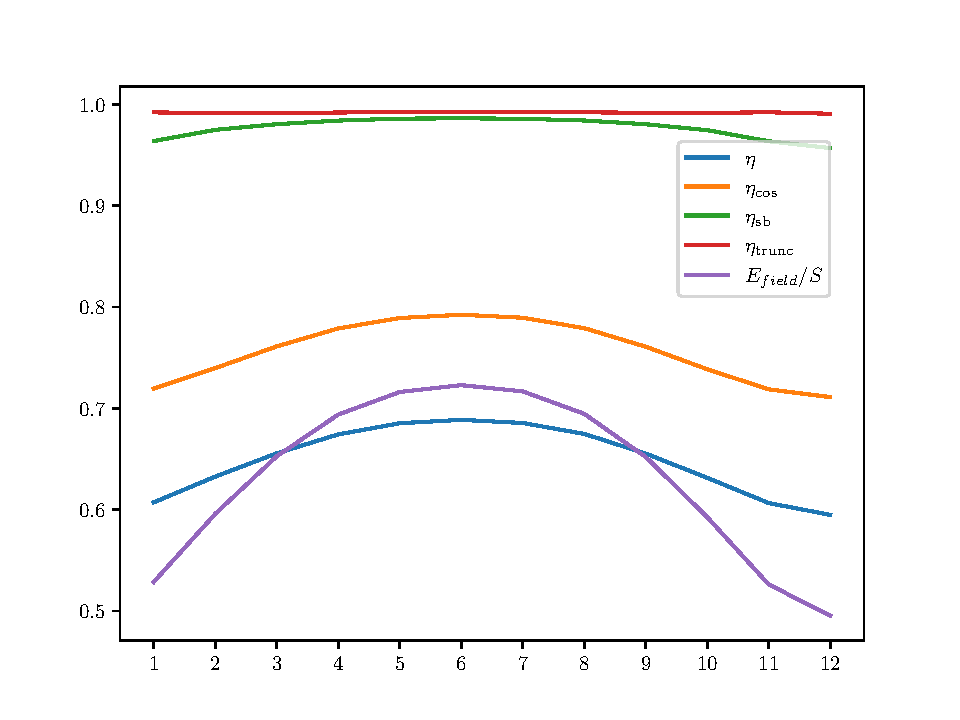
\includegraphics[scale = 0.5]{zhexiantu.pdf}
\caption{\kaishu 各个指标随月份变化折线图}
\end{figure}
%
\begin{figure}[H]
\centering
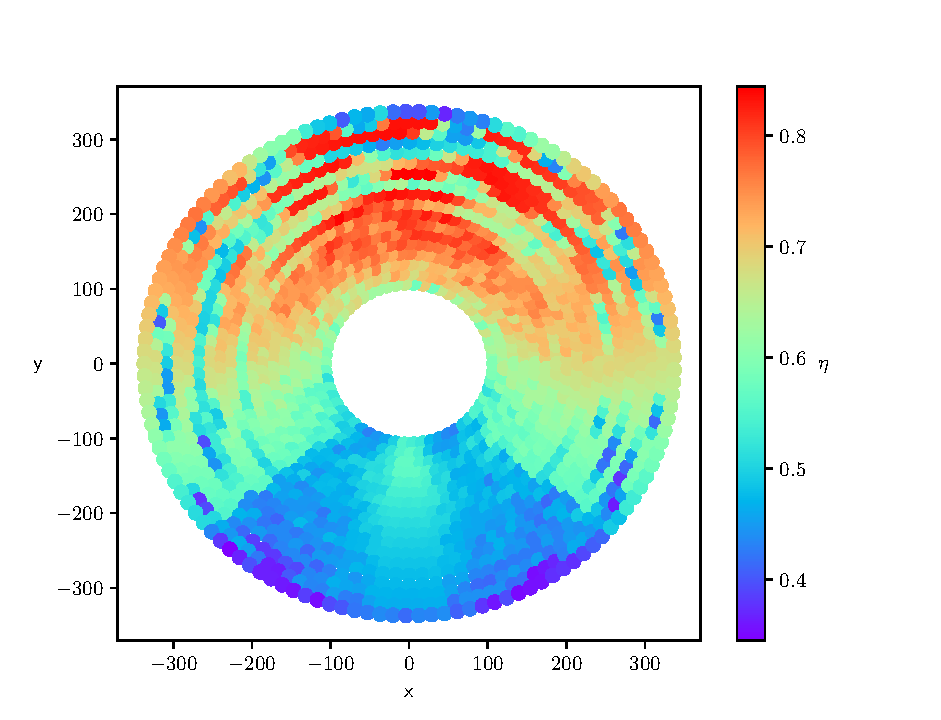
\includegraphics[scale =0.7]{rainbow.pdf}
\caption{\kaishu 春分{\rm 12:00}时分镜场内各个定日镜光学效率可视化结果}\label{rainbow}
\end{figure}
对于上述建立的模型,本文给出了在春分这一天的正午时刻下,计算定日镜场各个定日镜所对应的光学效率的分布。并做以下的合理性分析:
由图~\ref{rainbow} 可以看出,由于正午太阳光线在\(x\)轴方向上的分量为\(0\),所以此时定日场的左右两半的光学效率几乎是呈对称排布的,与实际情况相符;另外,对于这张分布图从南向北分析,可以看出,\(\eta\)大致呈现逐渐增大的变化趋势,这是由于对于吸收塔北面的定日镜而言,其法向量与太阳入射光线的法向量的夹角较小(如图~\ref{north_south} ),致使其余弦效率\(\eta_{\cos}\)相比南面的定日镜大,最终这种差异通过乘算作用于光学效率\(\eta\)上,与实际情况相符。综上,模型的合理性可以粗略地得证。
%
\begin{figure}[H]
\centering
\input north_south.tex
\caption{\kaishu 位于南北的定日镜的示意图}\label{north_south}
\end{figure}
\end{document}
